% Welcome! This is the unofficial University of Udine beamer template.

% See README.md for more informations about this template.

% This style has been developed following the "Manuale di Stile"
% (Style Manual) of the University of Udine. You can find the
% manual here: https://www.uniud.it/it/ateneo-uniud/ateneo-uniud/identita-visiva/manuali-immagine-stile/manuale-stile

% Note: for some reason, the RGB values specified in the manual
% do NOT render correctly in Beamer, so they have been redefined
% for this document using the high level chromo-optic deep neural 
% quantistic technology offered by Microsoft Paint's color picker.

% We defined four theme colors: UniBrown, UniBlue, UniGold
% and UniOrange. For example, to write some uniud-brownish
% text, just use: \textcolor{UniBrown}{Hello!}

% Note that [usenames,dvipsnames] is MANDATORY due to compatibility
% issues between tikz and xcolor packages.

\documentclass[usenames,dvipsnames]{beamer}
\usepackage[utf8]{inputenc}
\usepackage{verbatim}
\usepackage{multicol}
\usepackage{cases}
\usepackage{cancel}
\usetheme{uniud}
%set depth of Outline
\setcounter{tocdepth}{2}
%%% Bibliography
\usepackage[style=authoryear,backend=biber]{biblatex}
\addbibresource{bibliography.bib}

% Author names in publication list are consistent 
% i.e. name1 surname1, name2 surname2
% See https://tex.stackexchange.com/questions/106914/biblatex-does-not-reverse-the-first-and-last-names-of-the-second-author
\DeclareNameAlias{author}{first-last}

%%% Suppress biblatex annoying warning
\usepackage{silence}
\WarningFilter{biblatex}{Patching footnotes failed}

%%% Some useful commands
% pdf-friendly newline in links
\newcommand{\pdfnewline}{\texorpdfstring{\newline}{ }} 
% Fill the vertical space in a slide (to put text at the bottom)
\newcommand{\framefill}{\vskip0pt plus 1filll}


\title[IHEP SUSY Group Meeting]{Group Meeting}
\date[Oct 23, 2024]{Oct 23, 2024}
\author[Chengxin Liao]{
  Chengxin Liao
  \pdfnewline
  \texttt{lcx1937629829@icloud.com}
}
\institute{Department of Physics, Shandong University}

\begin{document}

\begin{frame}
\titlepage
\end{frame}

\begin{frame}{Outline}
\tableofcontents
\end{frame}

\section{C1N2ISR:double-check cutflow}
\begin{frame}
\frametitle{C1N2ISR:double-check cutflow}
Last week, I mistakenly put the yields file in merge dir, so it casued the difference in cutflow file.(The purple area represents the same data)

jiarong's cutflow(hhmet)
\begin{figure}
	\centering
	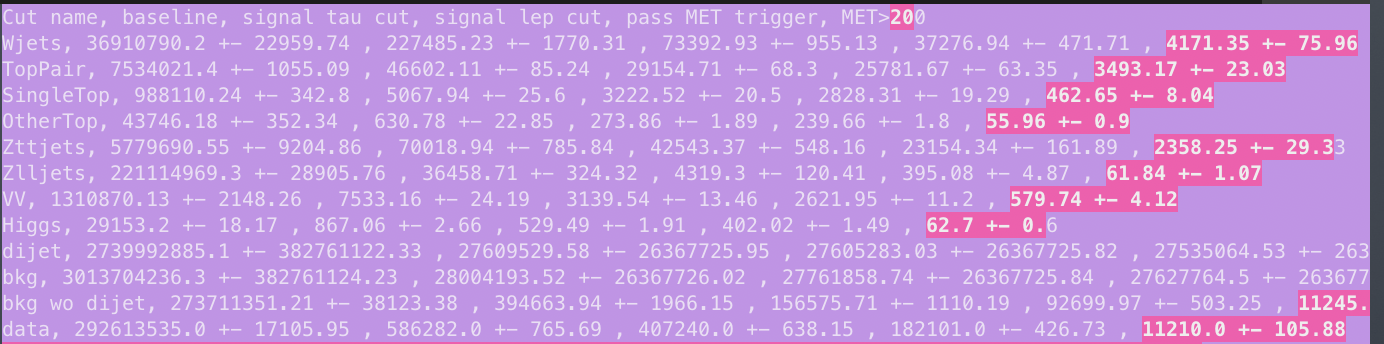
\includegraphics[width = 0.9\textwidth]{graphics/jiaronghhcutflow}
	\label{jiarong's hh cutflow}
\end{figure}
chengxin's cutflow
\begin{figure}
	\centering
	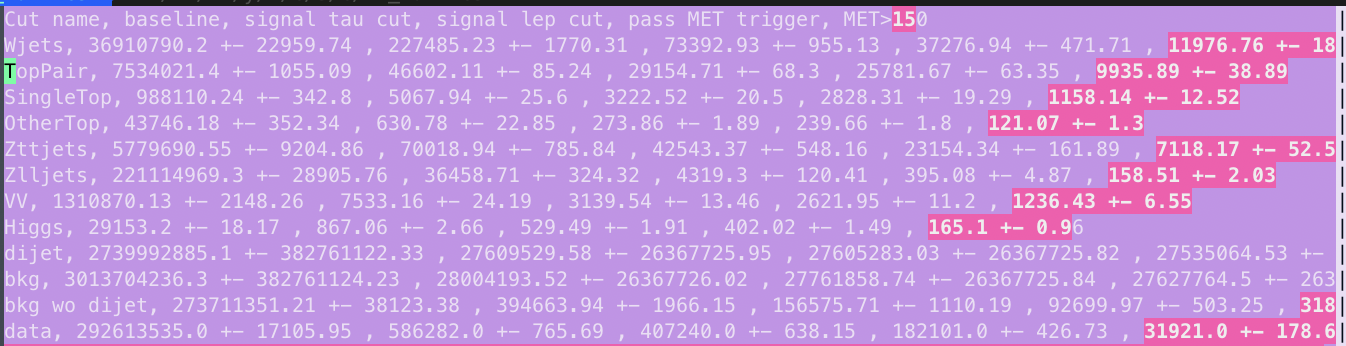
\includegraphics[width = 0.9\textwidth]{graphics/chengxinhhcutflow}
	\label{chengxin's hh cutflow}
\end{figure}

\end{frame}

\begin{frame}
\frametitle{C1N2ISR:double-check cutflow}
The purple area represents the same data

I already changed MET cut, but jobs still running, I will update when they all finished.

jiarong's cutflow(lhmet)
\begin{figure}
	\centering
	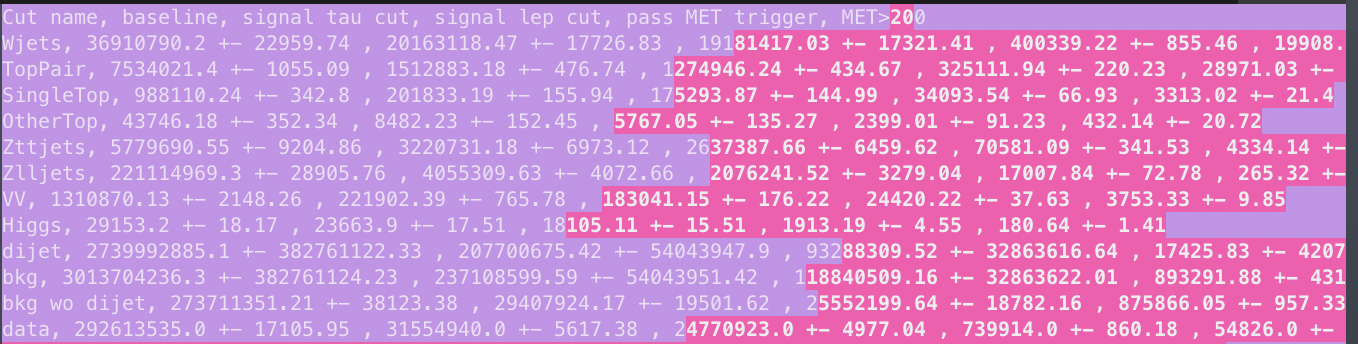
\includegraphics[width = 0.9\textwidth]{graphics/jiaronglhcutflow}
	\label{jiarong's lh cutflow}
\end{figure}
chengxin's cutflow
\begin{figure}
	\centering
	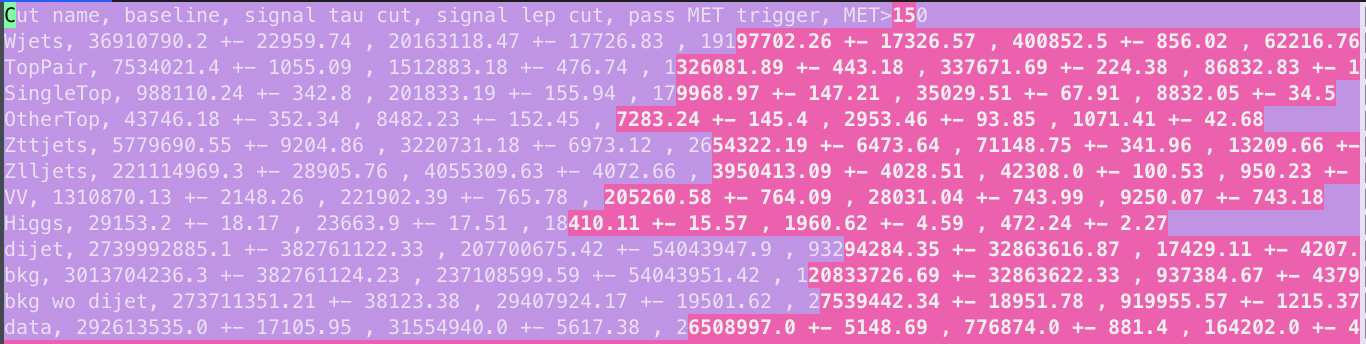
\includegraphics[width = 0.9\textwidth]{graphics/chengxinlhcutflow}
	\label{chengxin's lh cutflow}
\end{figure}
\end{frame}

\section{C1N2ISR: CutCount}
\begin{frame}
	\frametitle{C1N2ISR:CutCount}
	I just finish initial cutcount, but Zn seems too small. I need to refine step size and do a further optimization.(this for C1/N2 200p0/170p0)
	\begin{figure}
		\centering
		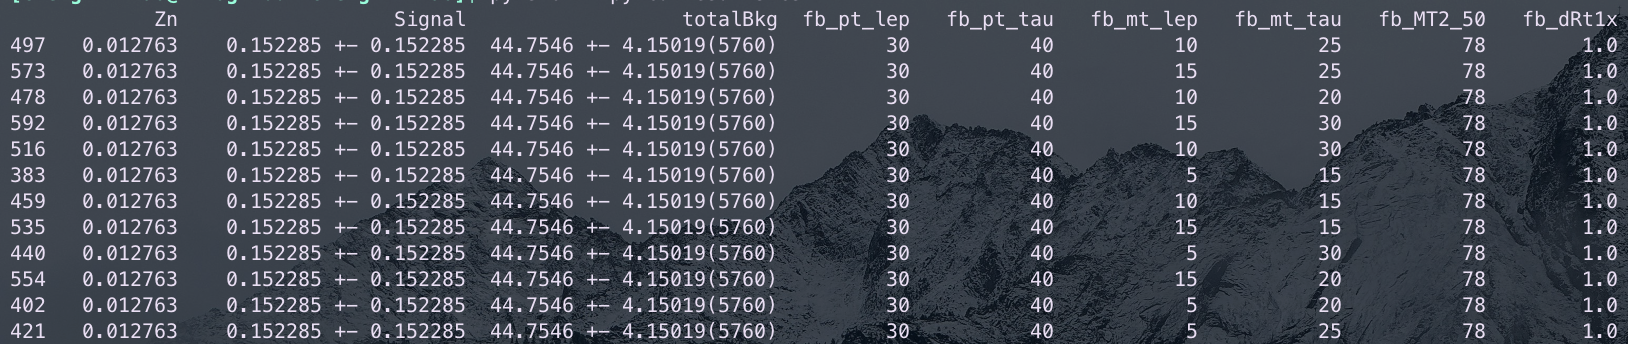
\includegraphics[width = 1.0\textwidth]{graphics/cutcount.png}
	\end{figure}
\end{frame}
\section{problems and TODO}
\begin{frame}
	\frametitle{problems and TODO}
	\framesubtitle{problems}
	
\end{frame}


\section{backup}
\subsection{var definition}
\begin{frame}
	\frametitle{backup}
	The definition of rapidity is $y = \frac{1}{2}ln\frac{E+p_z}{E-p_z}$. $\eta$ is pseudo-rapidity, $\eta = -ln(tan(\frac{\theta}{2})).$ It's easy to detect, and when speed close to light-speed, pseudo-rapidity nearly equal rapidity which can simplify detect of rapidity.
	
	$\phi$ is azimuthal angle of cylindrical coordinates
	
	R is angular distance, $R = \sqrt{\Delta\phi^2+\Delta\eta^2}$, R usually use to judge which particle belong to the same jet.
	
	METsig is Missing Transverse Energy Significance, $METsig = \frac{MET}{\sigma_{MET}}$, $\sigma_{MET}$ is the uncertainty of MET.
	
	Mll is the invariant between two taus, $Mll = \sqrt{(E_1 + E_2)^2 - (\vec{p_1}+\vec{p_2})^2}$
\end{frame}

\subsection{LH MC modeling}
\begin{frame}
\frametitle{C1N2ISR:MC modeling}
\framesubtitle{LH:\quad $\Delta\eta$}
% 第一行
    \begin{minipage}{0.32\textwidth}
        \centering
        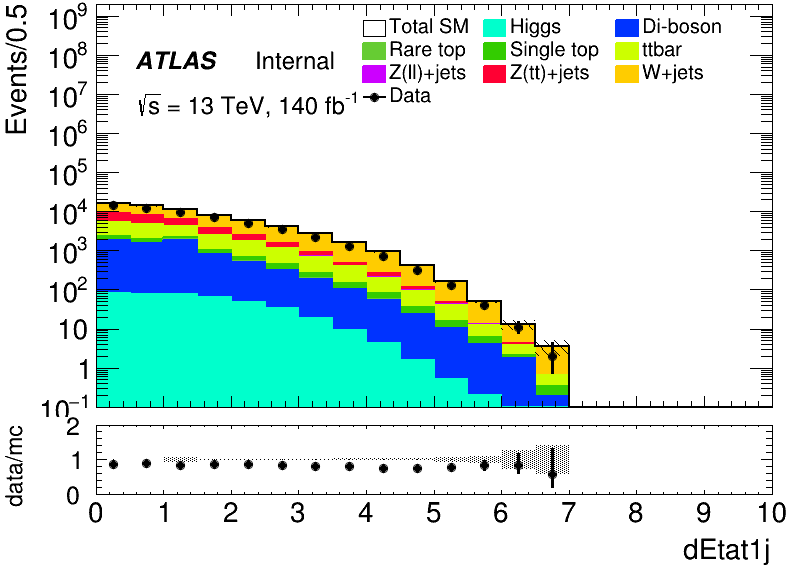
\includegraphics[width=\textwidth]{graphics/LH_met/LH_met_dEtat1j.png}
    \end{minipage}
    \hfill
    \begin{minipage}{0.32\textwidth}
        \centering
        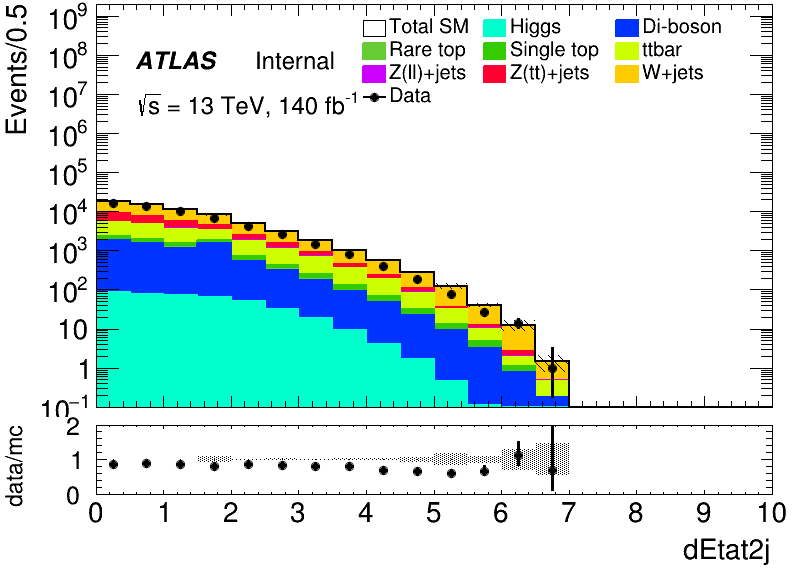
\includegraphics[width=\textwidth]{graphics/LH_met/LH_met_dEtat2j.png}
    \end{minipage}
    \hfill
    \begin{minipage}{0.32\textwidth}
        \centering
        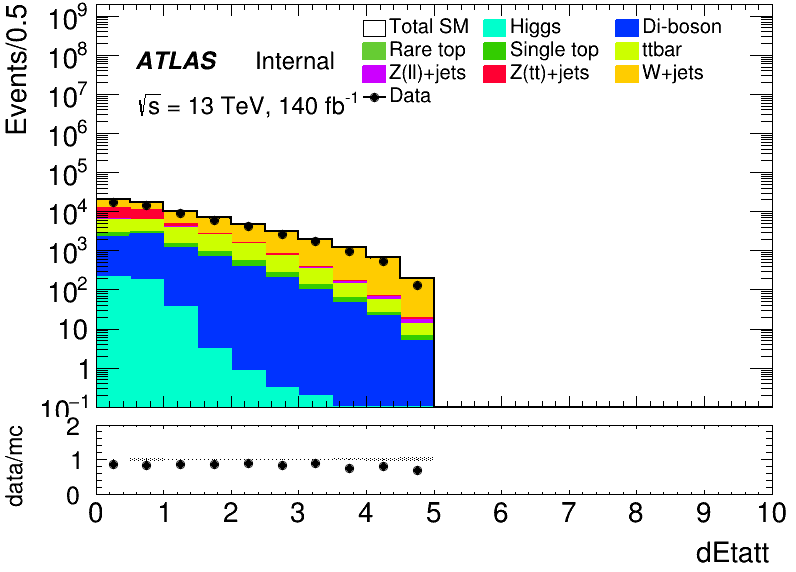
\includegraphics[width=\textwidth]{graphics/LH_met/LH_met_dEtatt.png}
    \end{minipage}
    
    \vspace{0.5cm} % 图片之间的竖直间距
    
    notice: t1 is leading tau, t2 is leading lep, j is leading jet, x is MET.
\end{frame}

\begin{frame}
\frametitle{C1N2ISR:MC modeling}
\framesubtitle{LH:\quad $\Delta\phi$}
% 第一行
    \begin{minipage}{0.32\textwidth}
        \centering
        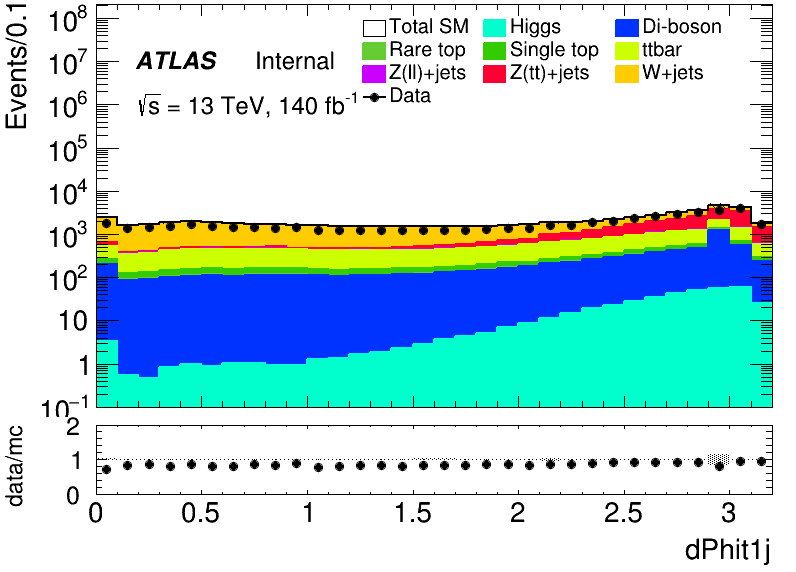
\includegraphics[width=\textwidth]{graphics/LH_met/LH_met_dPhit1j.png}
    \end{minipage}
    \hfill
    \begin{minipage}{0.32\textwidth}
        \centering
        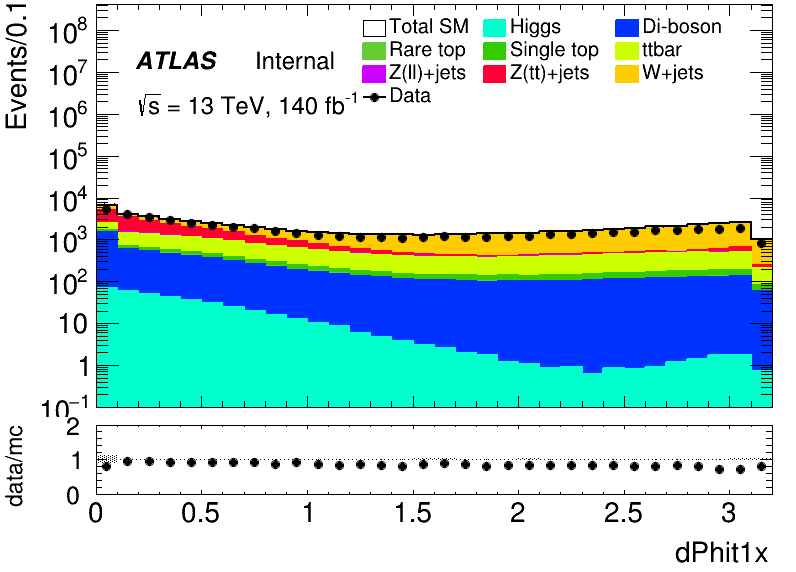
\includegraphics[width=\textwidth]{graphics/LH_met/LH_met_dPhit1x.png}
    \end{minipage}
    \hfill
    \begin{minipage}{0.32\textwidth}
        \centering
        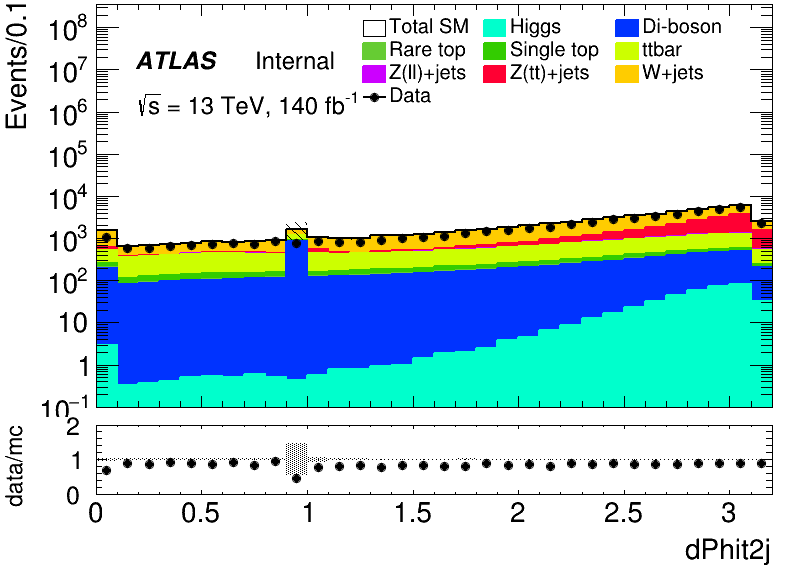
\includegraphics[width=\textwidth]{graphics/LH_met/LH_met_dPhit2j.png}
    \end{minipage}
    
    \vspace{0.5cm} % 图片之间的竖直间距

    % 第二行
    \begin{minipage}{0.32\textwidth}
        \centering
        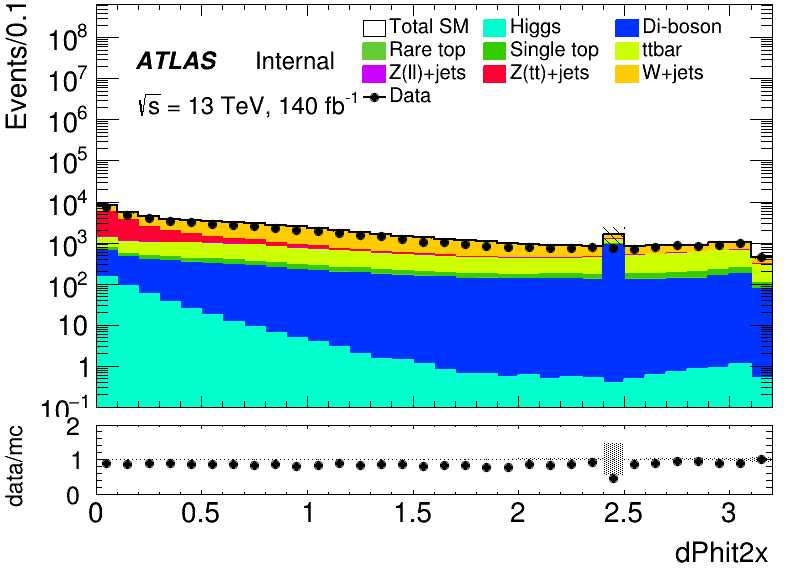
\includegraphics[width=\textwidth]{graphics/LH_met/LH_met_dPhit2x.png}
    \end{minipage}
    \hfill
    \begin{minipage}{0.32\textwidth}
        \centering
        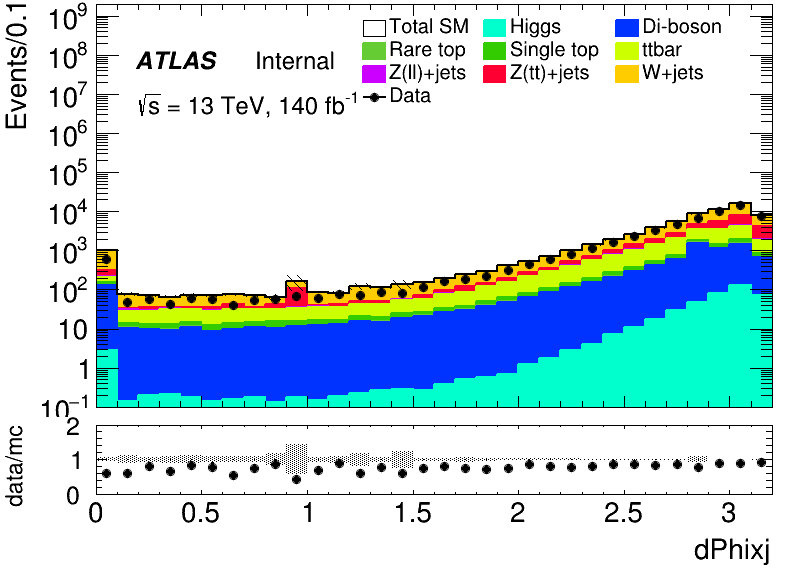
\includegraphics[width=\textwidth]{graphics/LH_met/LH_met_dPhixj.png}
    \end{minipage}
    \hfill
    \begin{minipage}{0.32\textwidth}
        \centering
        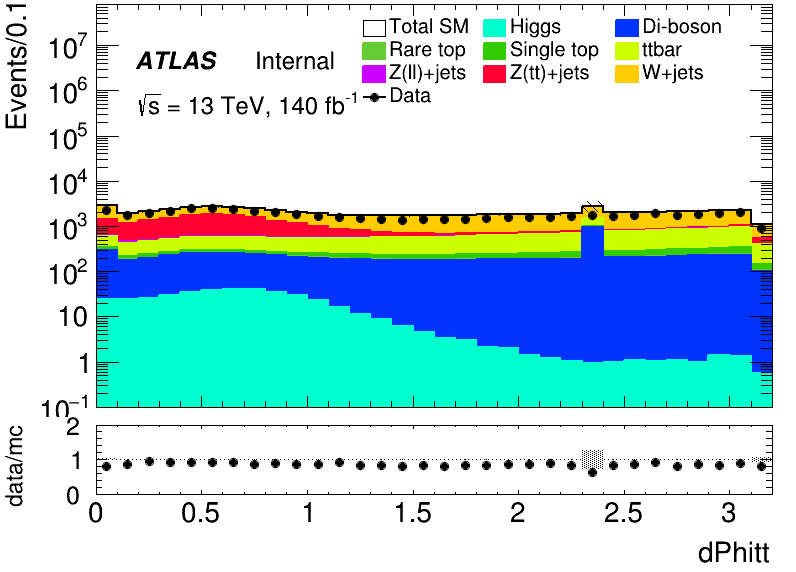
\includegraphics[width=\textwidth]{graphics/LH_met/LH_met_dPhitt.png}
    \end{minipage}
    notice: t1 is leading tau, t2 is leading lep, j is leading jet, x is MET.
\end{frame}

\begin{frame}
\frametitle{C1N2ISR:MC modeling}
\framesubtitle{LH:\quad $\Delta R$}
% 第一行
    \begin{minipage}{0.32\textwidth}
        \centering
        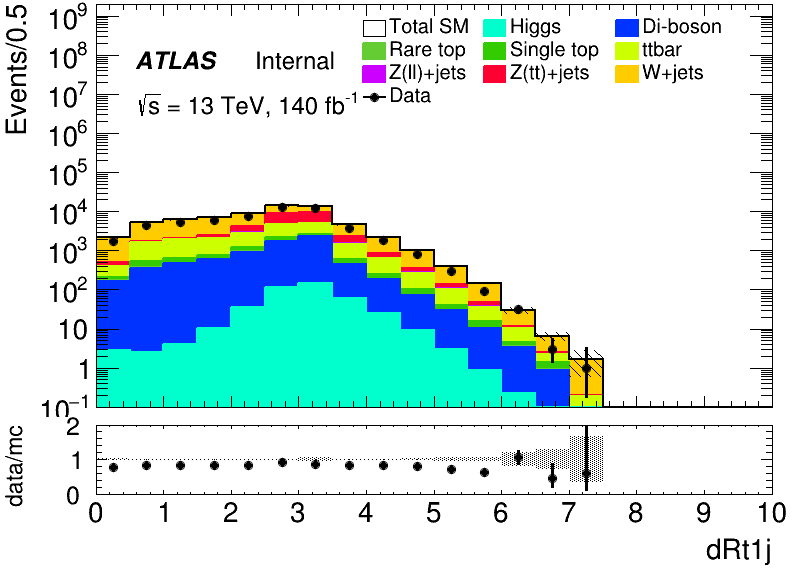
\includegraphics[width=\textwidth]{graphics/LH_met/LH_met_dRt1j.png}
    \end{minipage}
    \hfill
    \begin{minipage}{0.32\textwidth}
        \centering
        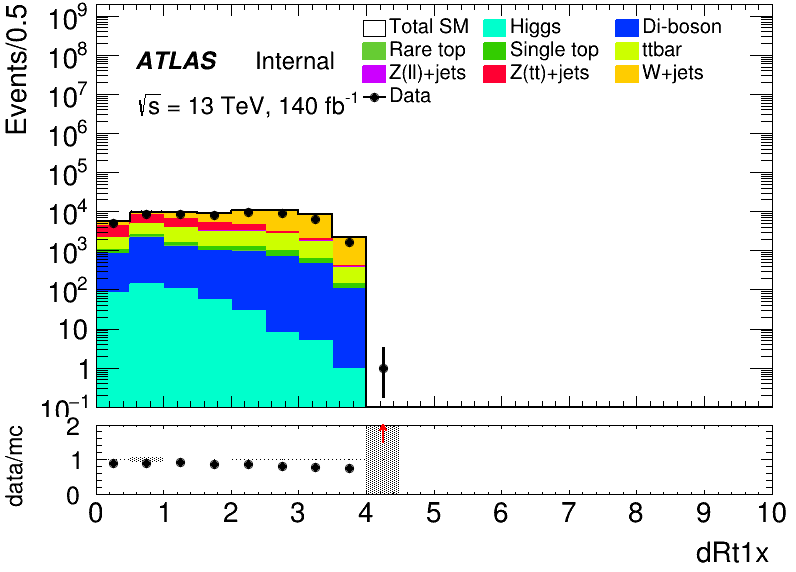
\includegraphics[width=\textwidth]{graphics/LH_met/LH_met_dRt1x.png}
    \end{minipage}
    \hfill
    \begin{minipage}{0.32\textwidth}
        \centering
        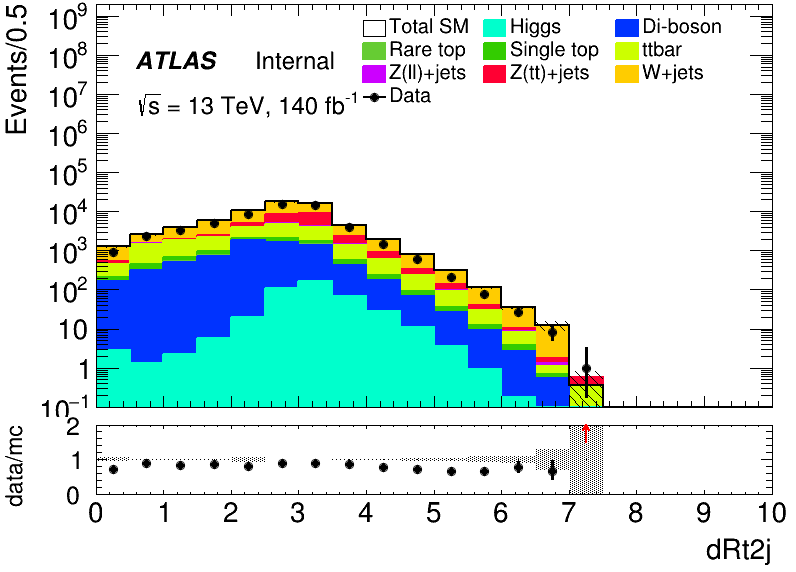
\includegraphics[width=\textwidth]{graphics/LH_met/LH_met_dRt2j.png}
    \end{minipage}
    
    \vspace{0.5cm} % 图片之间的竖直间距

    % 第二行
    \begin{minipage}{0.32\textwidth}
        \centering
        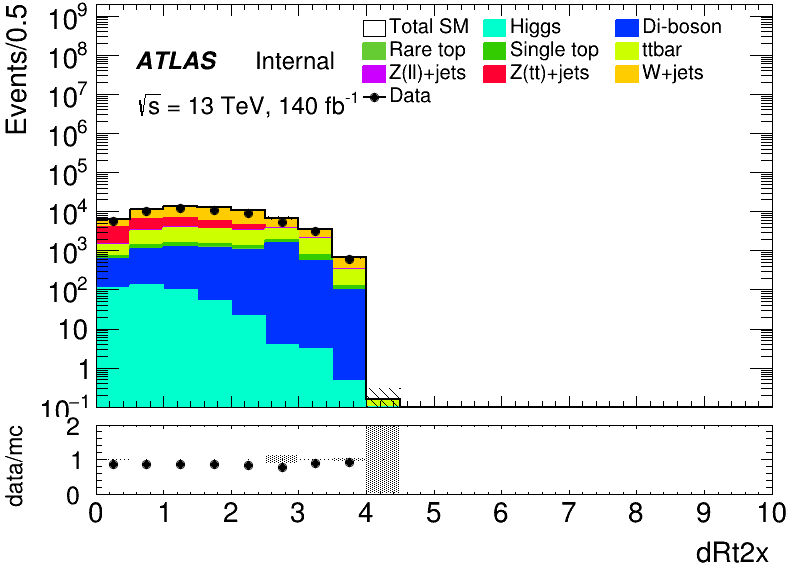
\includegraphics[width=\textwidth]{graphics/LH_met/LH_met_dRt2x.png}
    \end{minipage}
    \hfill
    \begin{minipage}{0.32\textwidth}
        \centering
        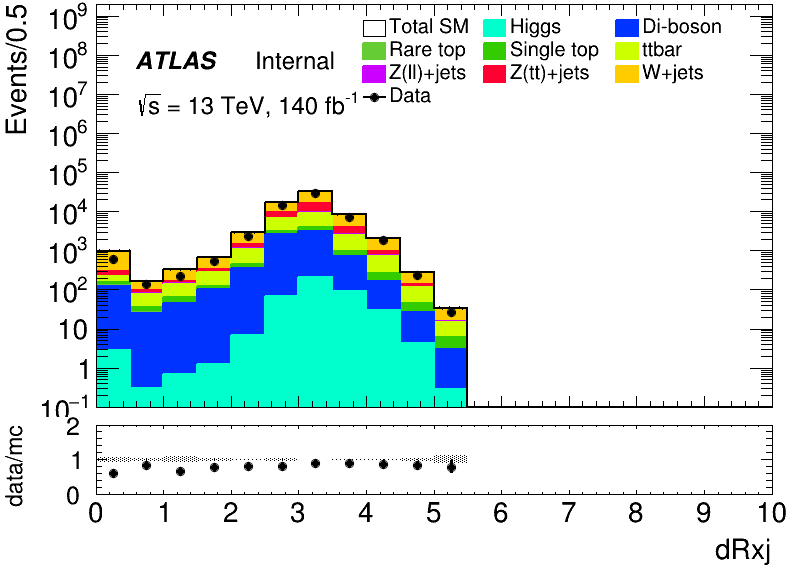
\includegraphics[width=\textwidth]{graphics/LH_met/LH_met_dRxj.png}
    \end{minipage}
    \hfill
    \begin{minipage}{0.32\textwidth}
        \centering
        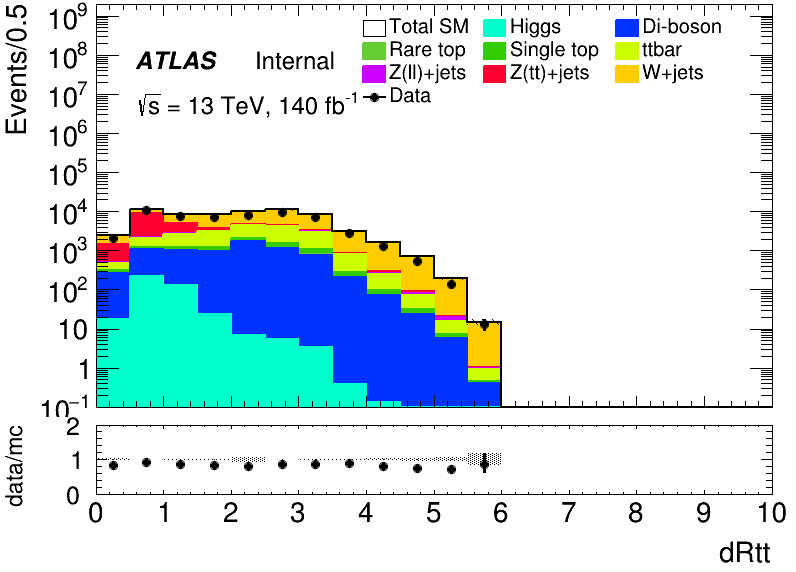
\includegraphics[width=\textwidth]{graphics/LH_met/LH_met_dRtt.png}
    \end{minipage}
    notice: t1 is leading tau, t2 is leading lep, j is leading jet, x is MET.
\end{frame}

\begin{frame}
\frametitle{C1N2ISR:MC modeling}
\framesubtitle{LH:$\quad\eta$}
% 第一行
    \begin{minipage}{0.32\textwidth}
        \centering
        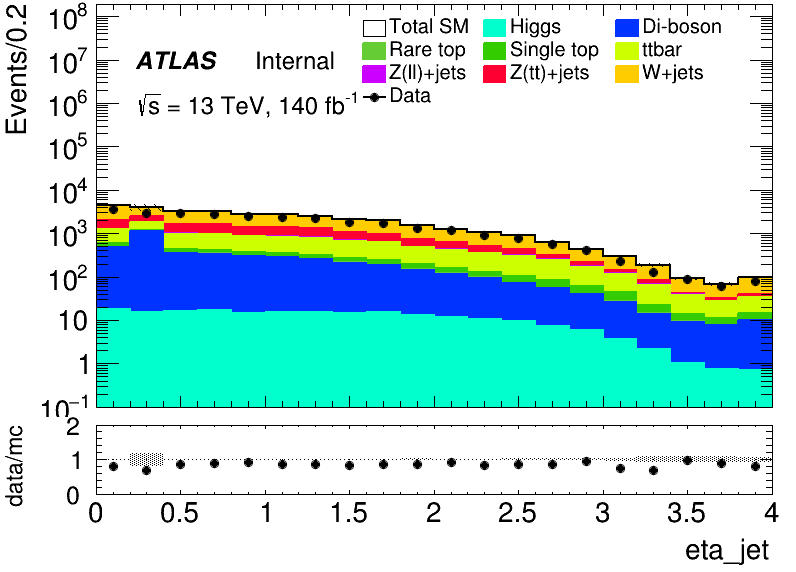
\includegraphics[width=\textwidth]{graphics/LH_met/LH_met_eta_jet.png}
    \end{minipage}
    \hfill
    \begin{minipage}{0.32\textwidth}
        \centering
        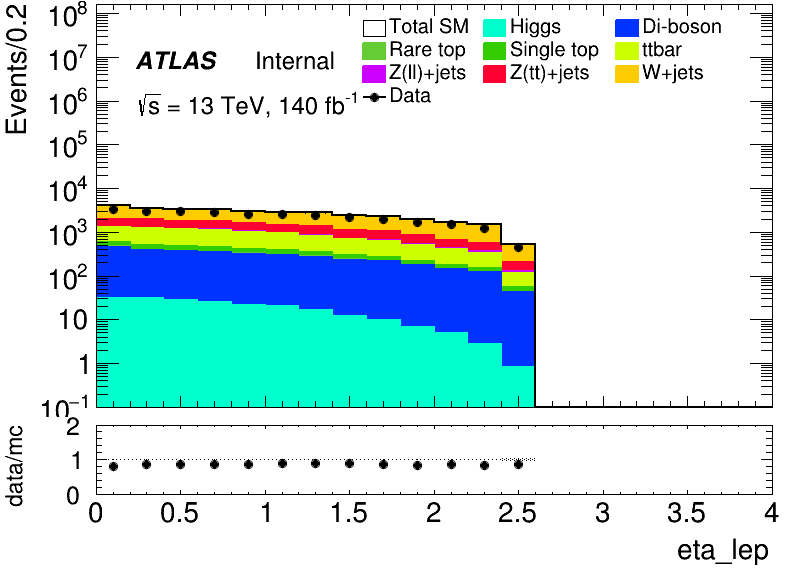
\includegraphics[width=\textwidth]{graphics/LH_met/LH_met_eta_lep.png}
    \end{minipage}
    \hfill
    \begin{minipage}{0.32\textwidth}
        \centering
        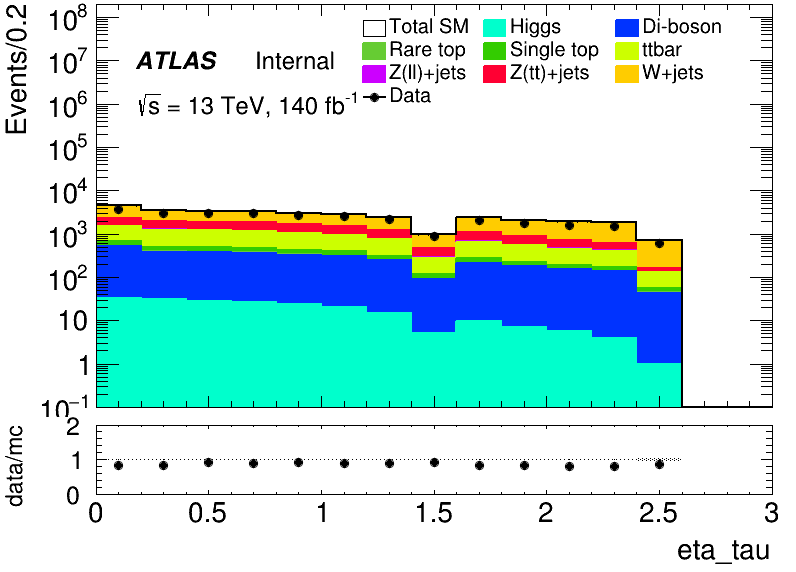
\includegraphics[width=\textwidth]{graphics/LH_met/LH_met_eta_tau.png}
    \end{minipage}
\end{frame}

\begin{frame}
\frametitle{C1N2ISR:MC modeling}
\framesubtitle{LH:\quad $p_t$}
% 第一行
    \begin{minipage}{0.32\textwidth}
        \centering
        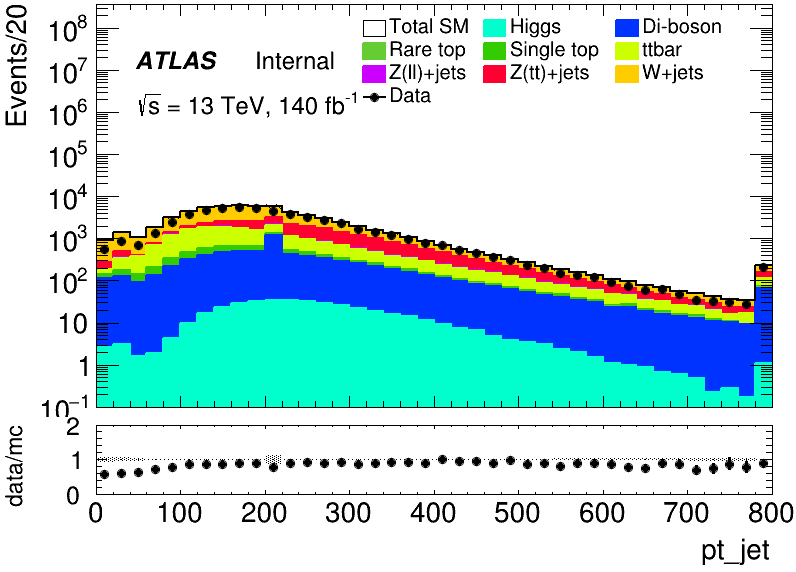
\includegraphics[width=\textwidth]{graphics/LH_met/LH_met_pt_jet.png}
    \end{minipage}
    \hfill
    \begin{minipage}{0.32\textwidth}
        \centering
        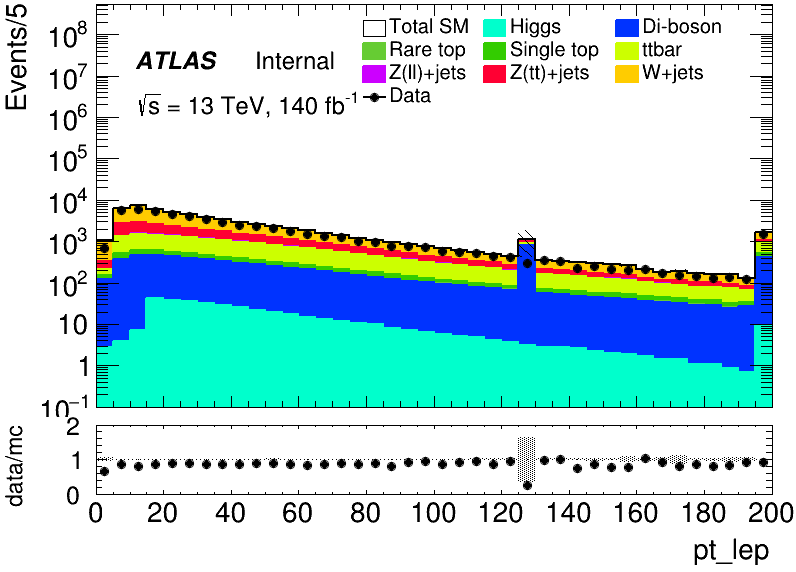
\includegraphics[width=\textwidth]{graphics/LH_met/LH_met_pt_lep.png}
    \end{minipage}
    \hfill
    \begin{minipage}{0.32\textwidth}
        \centering
        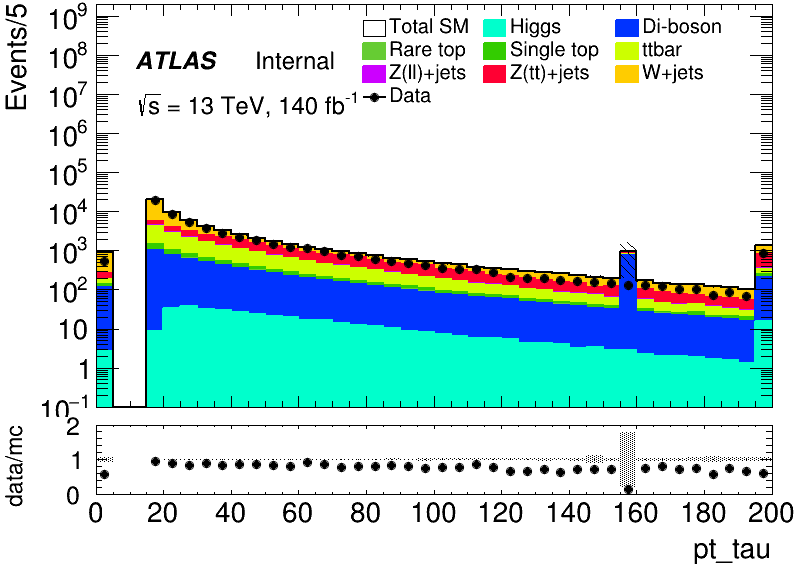
\includegraphics[width=\textwidth]{graphics/LH_met/LH_met_pt_tau.png}
    \end{minipage}
    
    \vspace{0.5cm} % 图片之间的竖直间距
\end{frame}

\begin{frame}
\frametitle{C1N2ISR:MC modeling}
\framesubtitle{LH:\quad num}
% 第一行
    \begin{minipage}{0.32\textwidth}
        \centering
        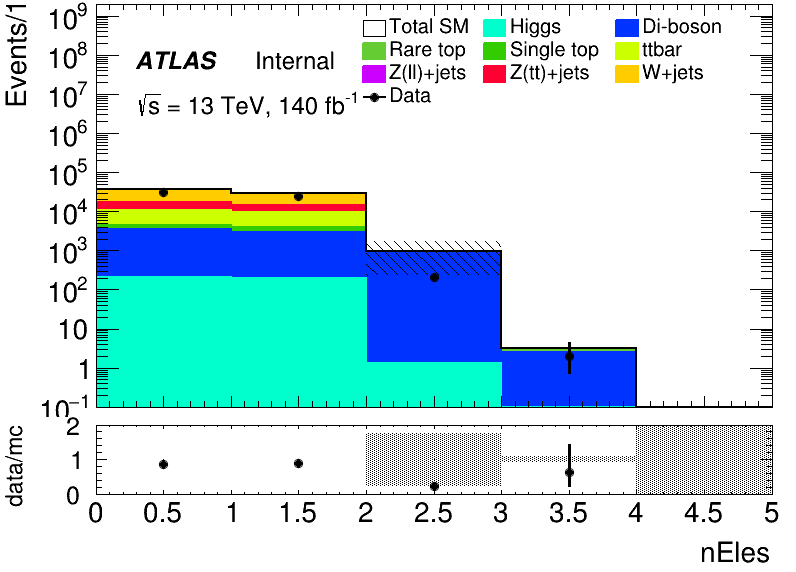
\includegraphics[width=\textwidth]{graphics/LH_met/LH_met_nEles.png}
    \end{minipage}
    \hfill
    \begin{minipage}{0.32\textwidth}
        \centering
        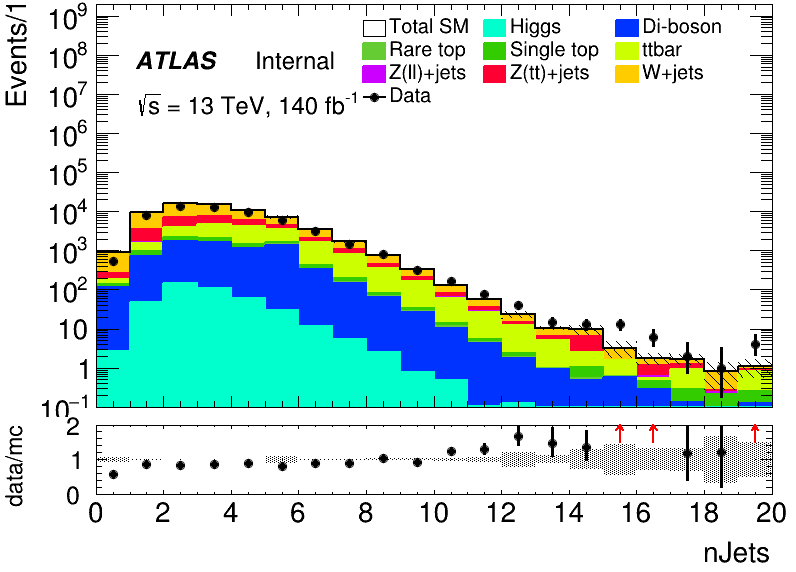
\includegraphics[width=\textwidth]{graphics/LH_met/LH_met_nJets.png}
    \end{minipage}
    \hfill
    \begin{minipage}{0.32\textwidth}
        \centering
        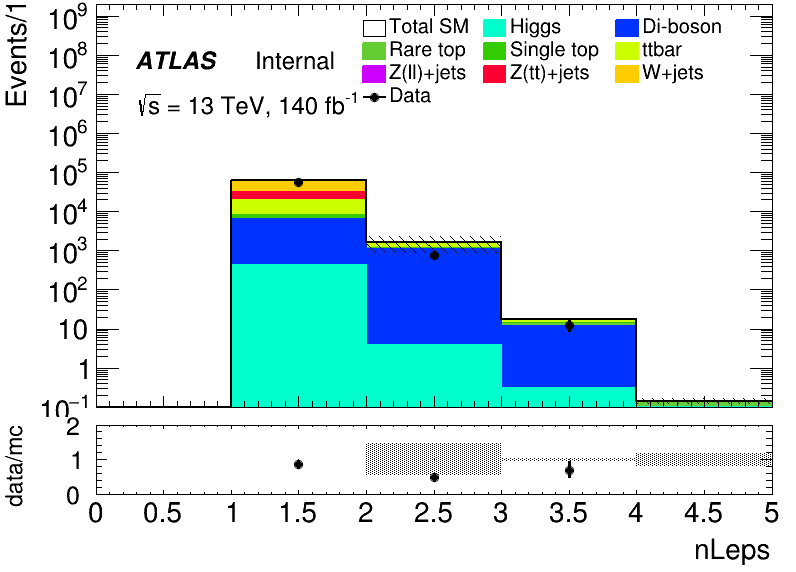
\includegraphics[width=\textwidth]{graphics/LH_met/LH_met_nLeps.png}
    \end{minipage}
    
    \vspace{0.5cm} % 图片之间的竖直间距

    % 第二行
    \begin{minipage}{0.32\textwidth}
        \centering
        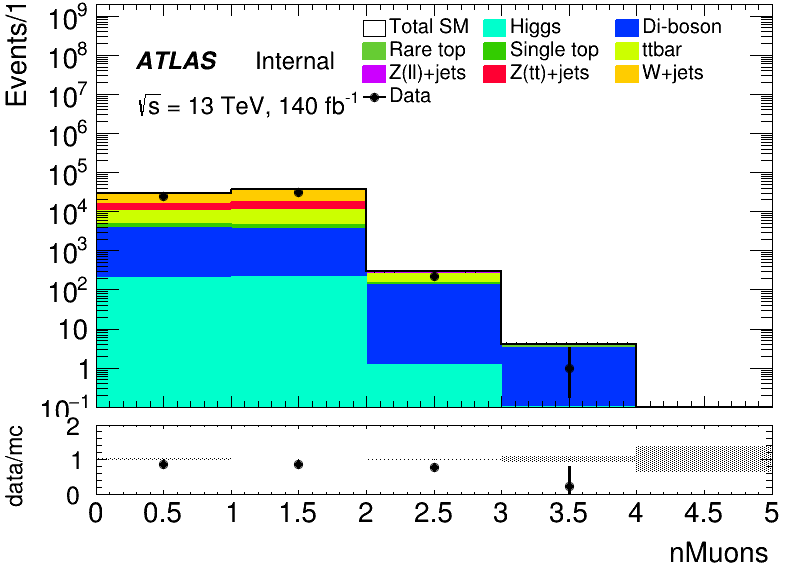
\includegraphics[width=\textwidth]{graphics/LH_met/LH_met_nMuons.png}
    \end{minipage}
    \hfill
    \begin{minipage}{0.32\textwidth}
        \centering
        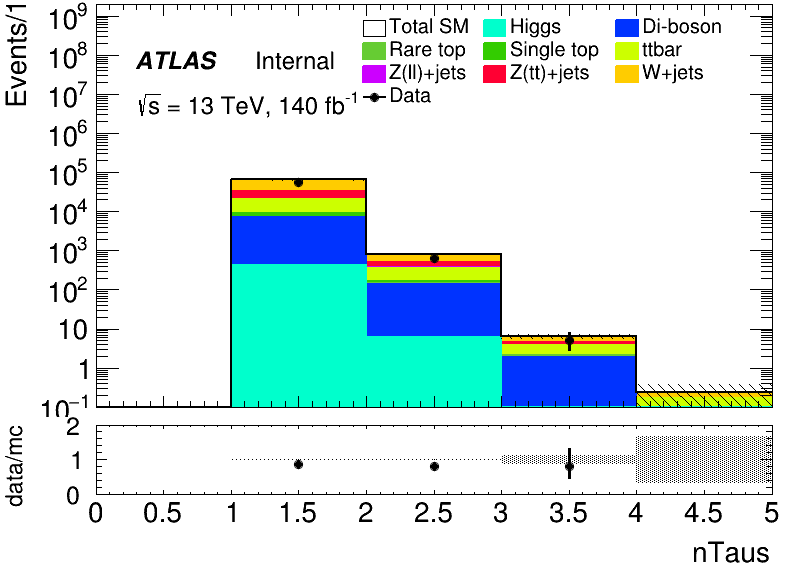
\includegraphics[width=\textwidth]{graphics/LH_met/LH_met_nTaus.png}
    \end{minipage}
    \hfill
    \begin{minipage}{0.32\textwidth}
        \centering
        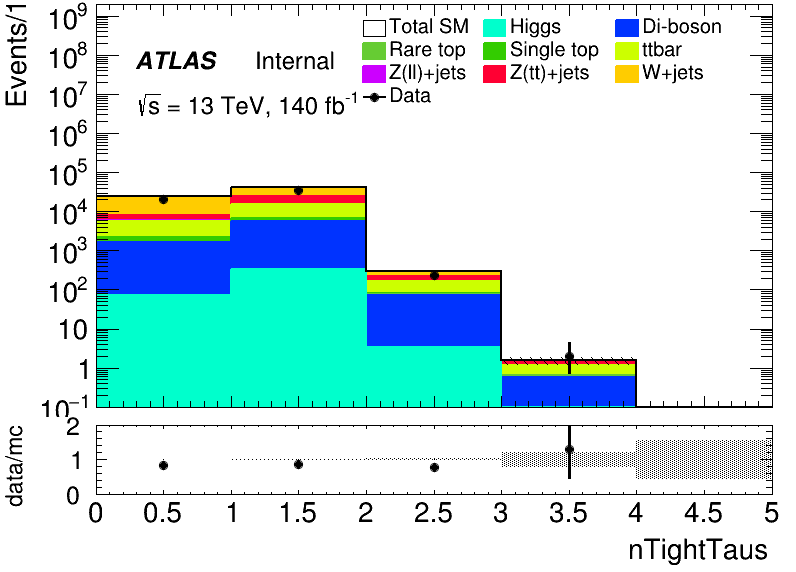
\includegraphics[width=\textwidth]{graphics/LH_met/LH_met_nTightTaus.png}
    \end{minipage}
\end{frame}

\begin{frame}
\frametitle{C1N2ISR:MC modeling}
\framesubtitle{LH:\quad transverse mass}
% 第一行
    \begin{minipage}{0.32\textwidth}
        \centering
        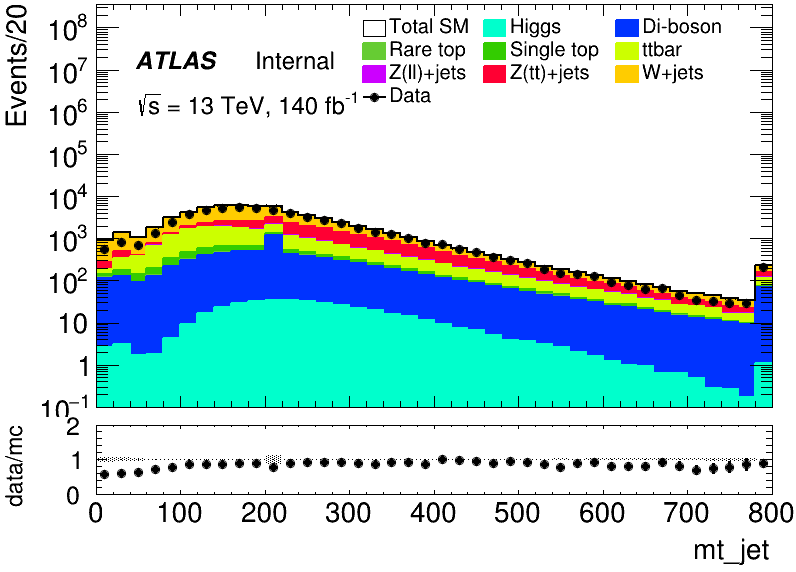
\includegraphics[width=\textwidth]{graphics/LH_met/LH_met_mt_jet.png}
    \end{minipage}
    \hfill
    \begin{minipage}{0.32\textwidth}
        \centering
        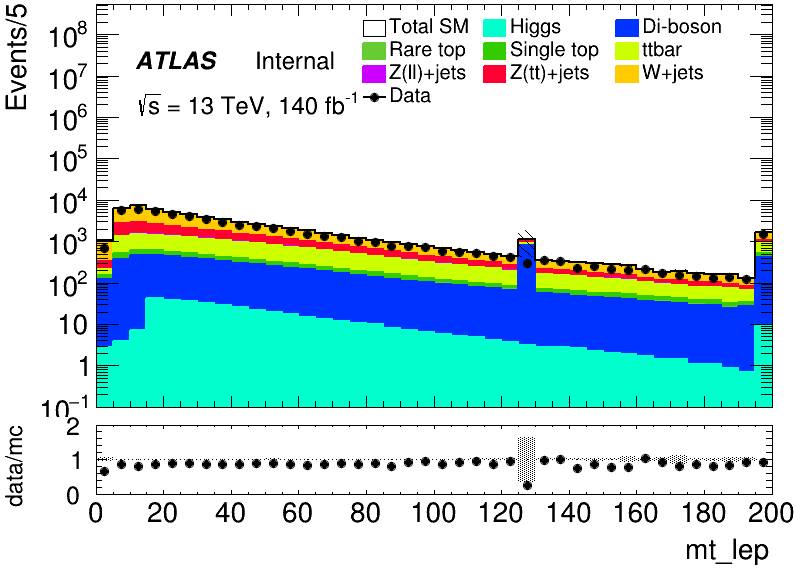
\includegraphics[width=\textwidth]{graphics/LH_met/LH_met_mt_lep.png}
    \end{minipage}
    \hfill
    \begin{minipage}{0.32\textwidth}
        \centering
        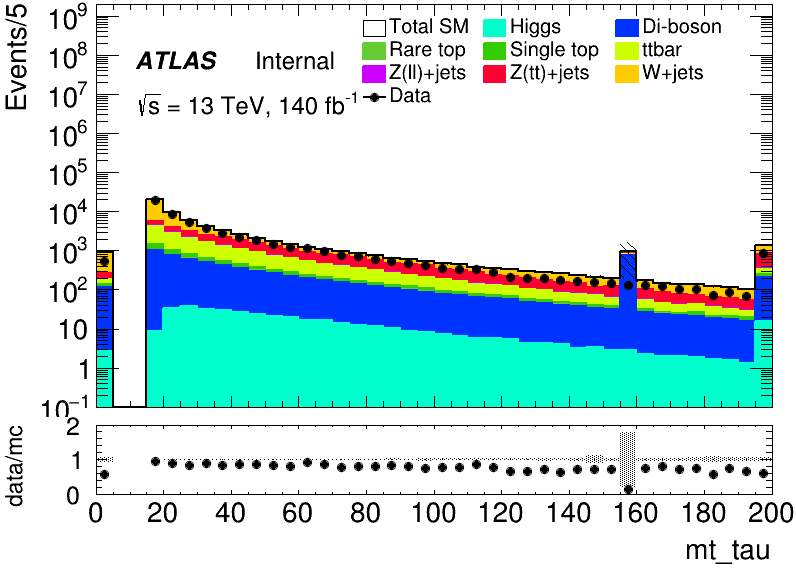
\includegraphics[width=\textwidth]{graphics/LH_met/LH_met_mt_tau.png}
    \end{minipage}
    
    \vspace{0.5cm} % 图片之间的竖直间距

    % 第二行
    \begin{minipage}{0.32\textwidth}
        \centering
        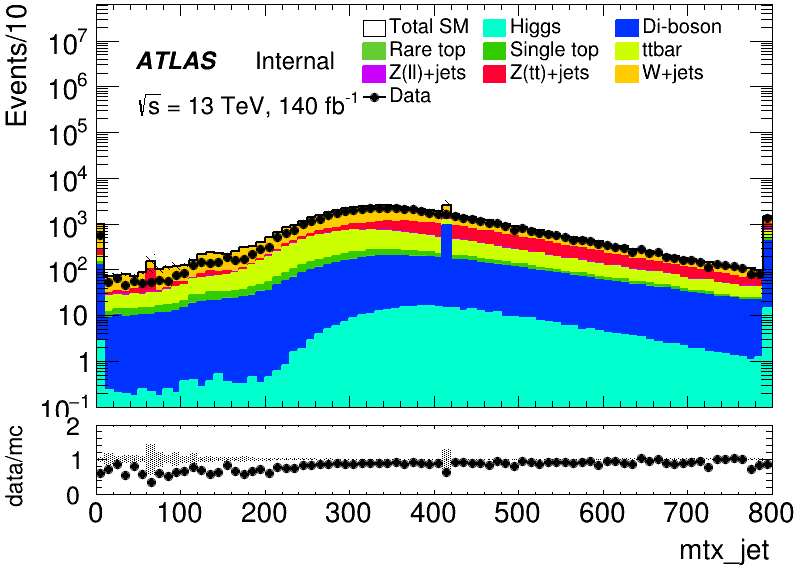
\includegraphics[width=\textwidth]{graphics/LH_met/LH_met_mtx_jet.png}
    \end{minipage}
        \hfill
    \begin{minipage}{0.32\textwidth}
        \centering
        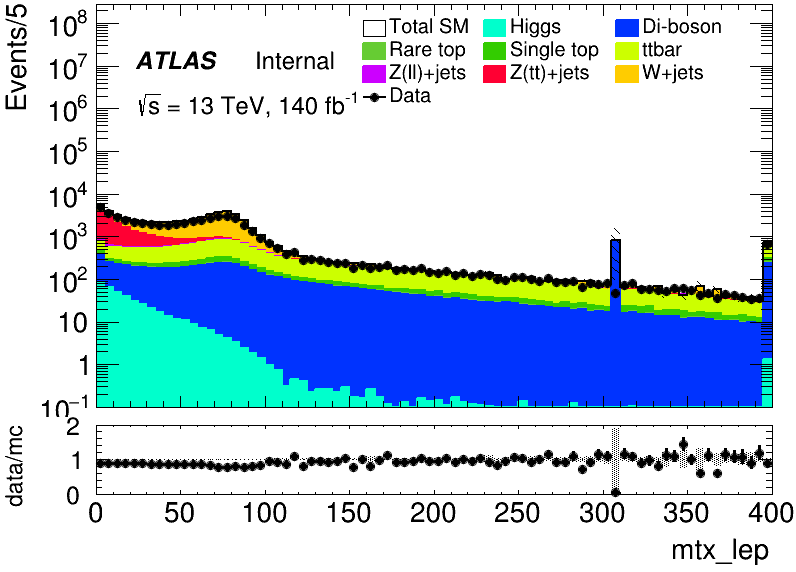
\includegraphics[width=\textwidth]{graphics/LH_met/LH_met_mtx_lep.png}
    \end{minipage}
    \hfill
    \begin{minipage}{0.32\textwidth}
        \centering
        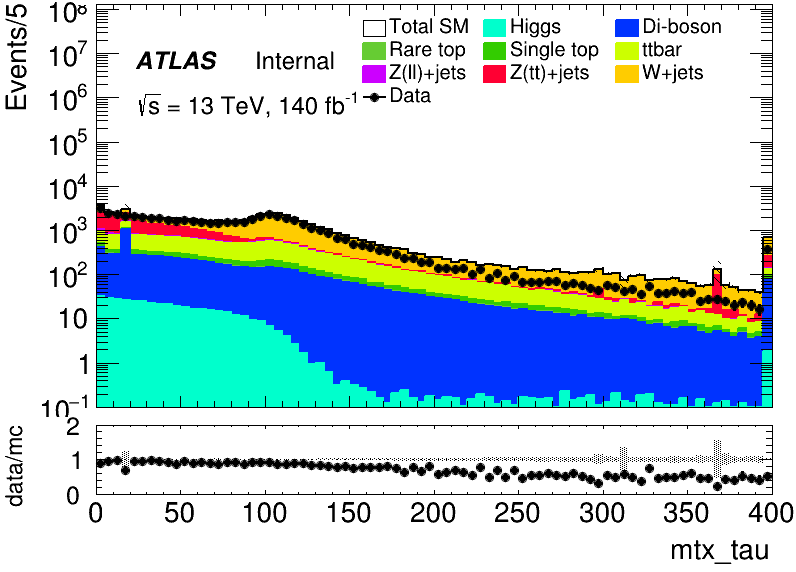
\includegraphics[width=\textwidth]{graphics/LH_met/LH_met_mtx_tau.png}
    \end{minipage}
    notice: mtx is the projection of MT in METvec.
\end{frame}
\begin{frame}
\frametitle{C1N2ISR:MC modeling}
\framesubtitle{LH:\quad stranverse mass, invariant mass, MET}
% 第一行
    \begin{minipage}{0.32\textwidth}
        \centering
        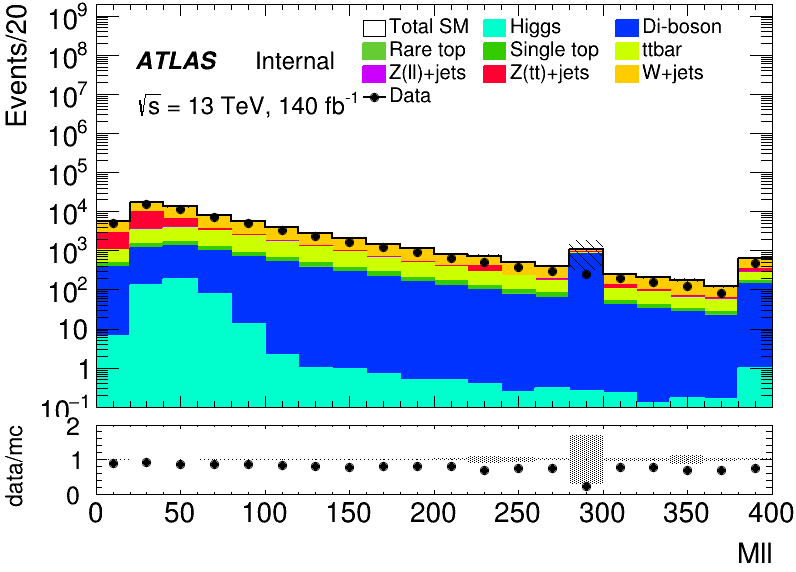
\includegraphics[width=\textwidth]{graphics/LH_met/LH_met_Mll.png}
    \end{minipage}
    \hfill
    \begin{minipage}{0.32\textwidth}
        \centering
        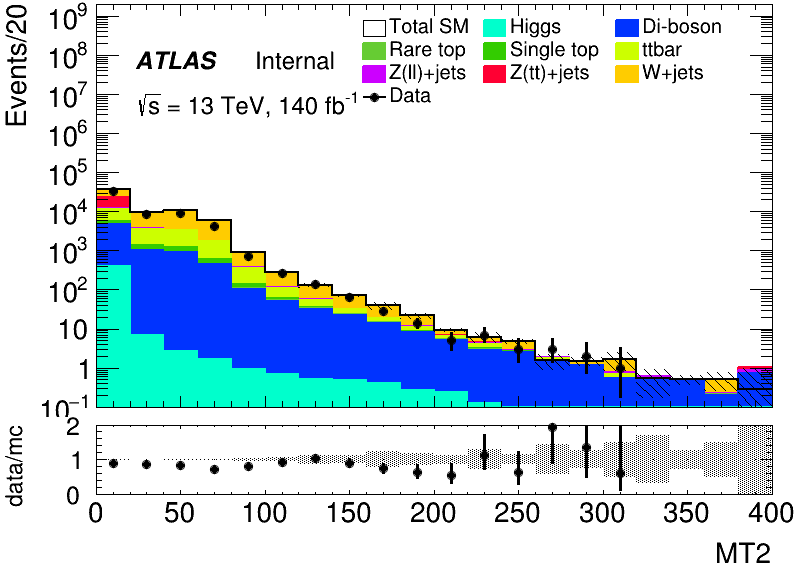
\includegraphics[width=\textwidth]{graphics/LH_met/LH_met_MT2.png}
    \end{minipage}
    \hfill
%    \begin{minipage}{0.32\textwidth}
%        \centering
%        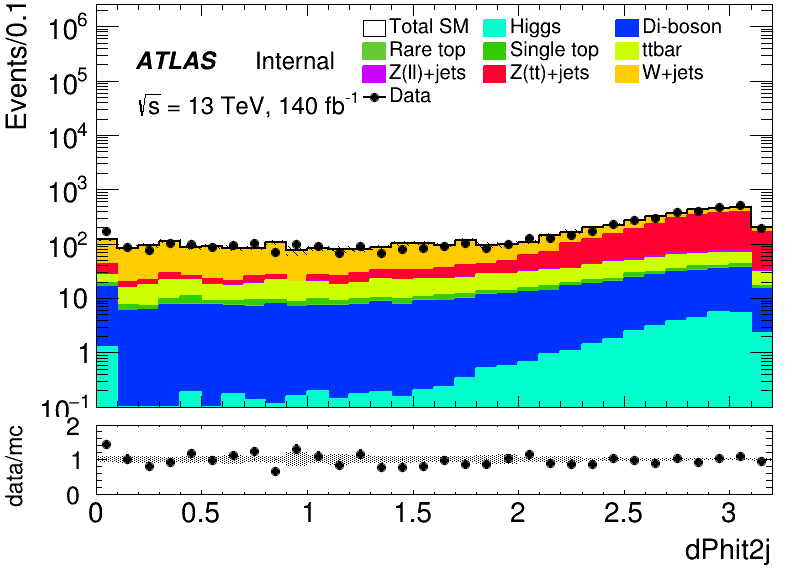
\includegraphics[width=\textwidth]{graphics/H_met/H_met_dPhit2j.png}
%    \end{minipage}
    
    \vspace{0.5cm} % 图片之间的竖直间距

    % 第二行
    \begin{minipage}{0.32\textwidth}
        \centering
        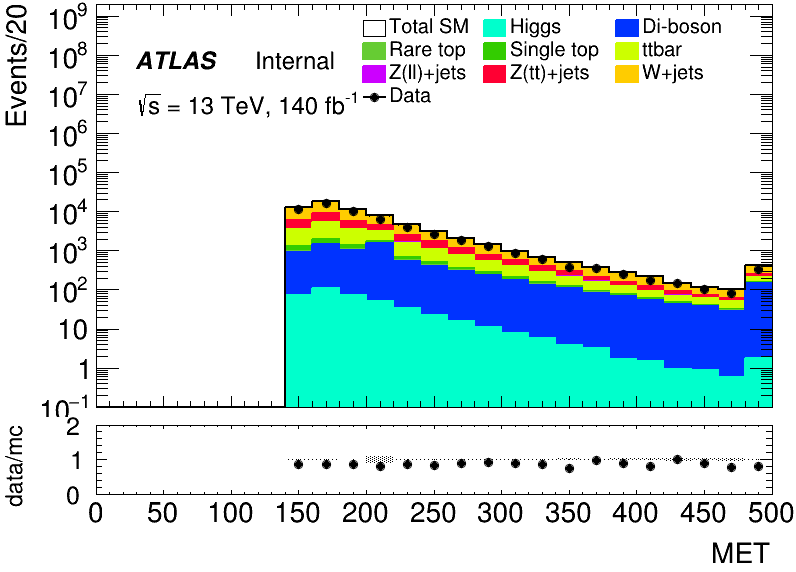
\includegraphics[width=\textwidth]{graphics/LH_met/LH_met_MET.png}
    \end{minipage}
    \hfill
    \begin{minipage}{0.32\textwidth}
        \centering
        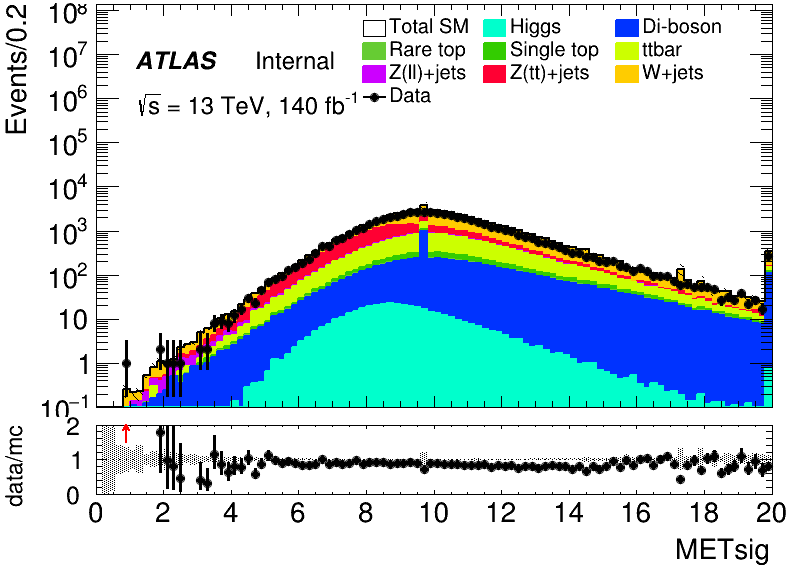
\includegraphics[width=\textwidth]{graphics/LH_met/LH_met_METsig.png}
    \end{minipage}
    \hfill
    
%    \begin{minipage}{0.32\textwidth}
%        \centering
%        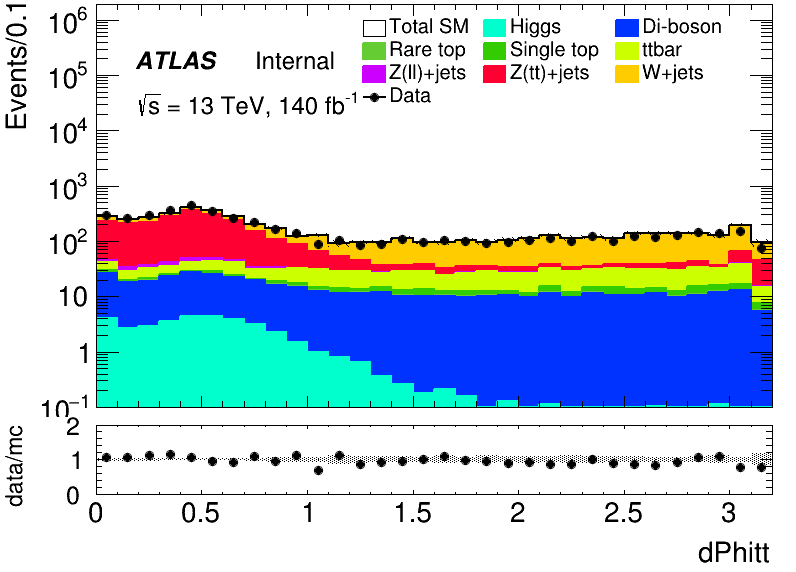
\includegraphics[width=\textwidth]{graphics/H_met/H_met_dPhitt.png}
%    \end{minipage}

\end{frame}

\subsection{HH MC modeling}
\begin{frame}
\frametitle{C1N2ISR:MC modeling}
\framesubtitle{HH:\quad $\Delta\eta$}
% 第一行
    \begin{minipage}{0.32\textwidth}
        \centering
        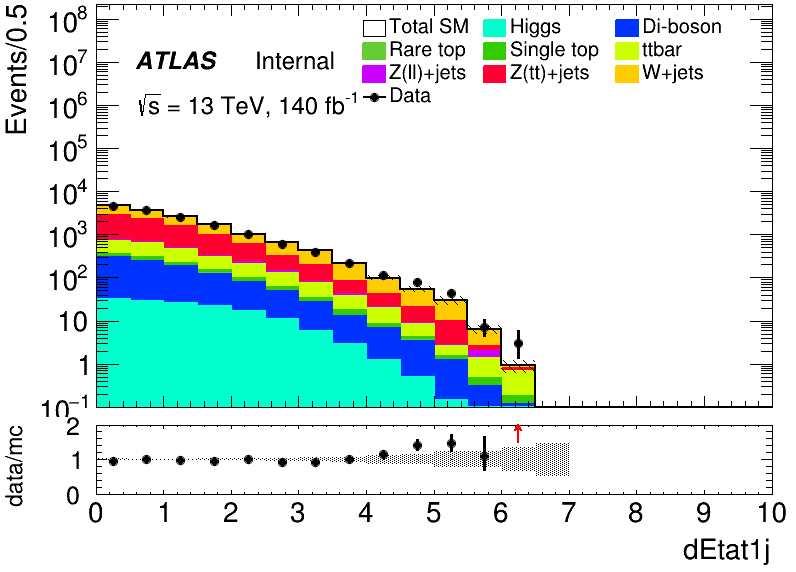
\includegraphics[width=\textwidth]{graphics/HH_met/HH_met_dEtat1j.png}
    \end{minipage}
    \hfill
    \begin{minipage}{0.32\textwidth}
        \centering
        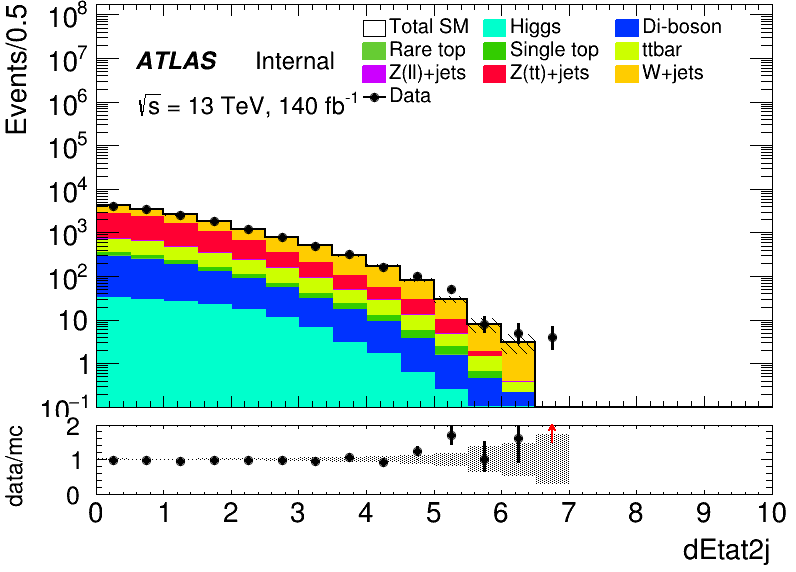
\includegraphics[width=\textwidth]{graphics/HH_met/HH_met_dEtat2j.png}
    \end{minipage}
    \hfill
    \begin{minipage}{0.32\textwidth}
        \centering
        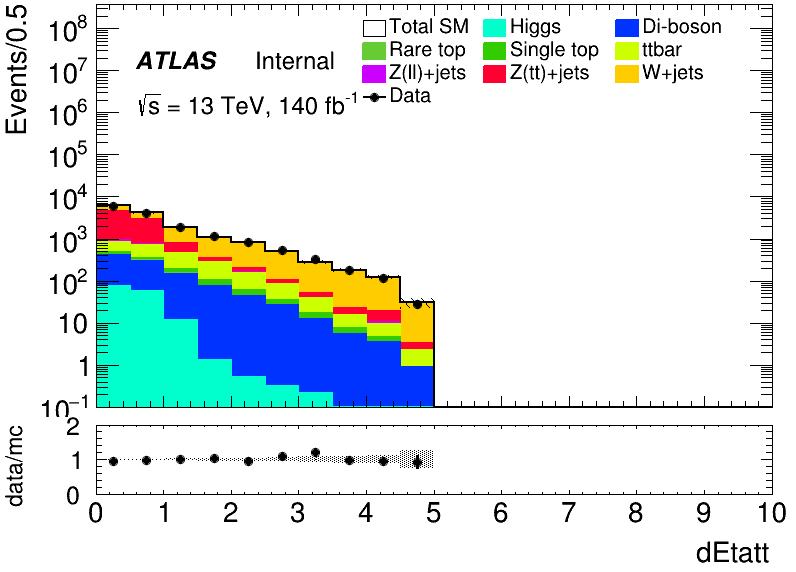
\includegraphics[width=\textwidth]{graphics/HH_met/HH_met_dEtatt.png}
    \end{minipage}
    
    \vspace{0.5cm} % 图片之间的竖直间距\
    notice: t1 is leading tau, t2 is next leading tau, j is leading jet, x is MET.
\end{frame}

\begin{frame}
\frametitle{C1N2ISR:MC modeling}
\framesubtitle{HH:\quad $\Delta\phi$}
% 第一行
    \begin{minipage}{0.32\textwidth}
        \centering
        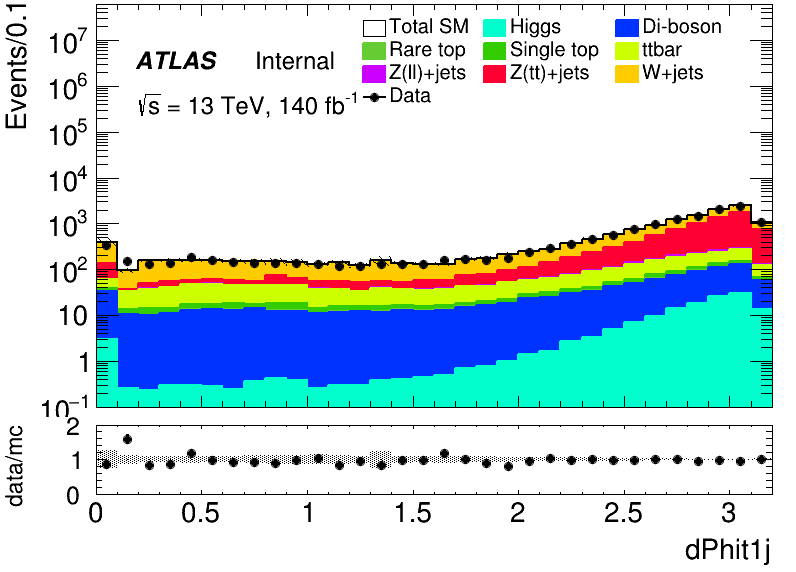
\includegraphics[width=\textwidth]{graphics/HH_met/HH_met_dPhit1j.png}
    \end{minipage}
    \hfill
    \begin{minipage}{0.32\textwidth}
        \centering
        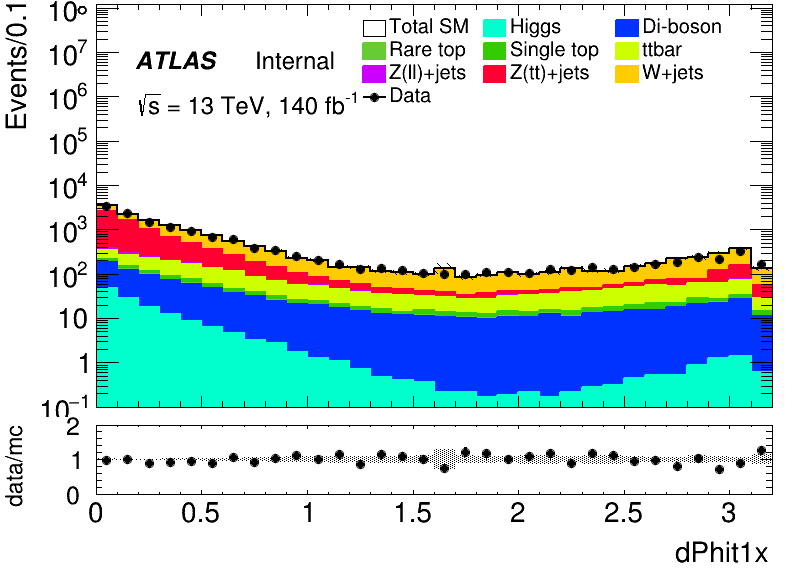
\includegraphics[width=\textwidth]{graphics/HH_met/HH_met_dPhit1x.png}
    \end{minipage}
    \hfill
    \begin{minipage}{0.32\textwidth}
        \centering
        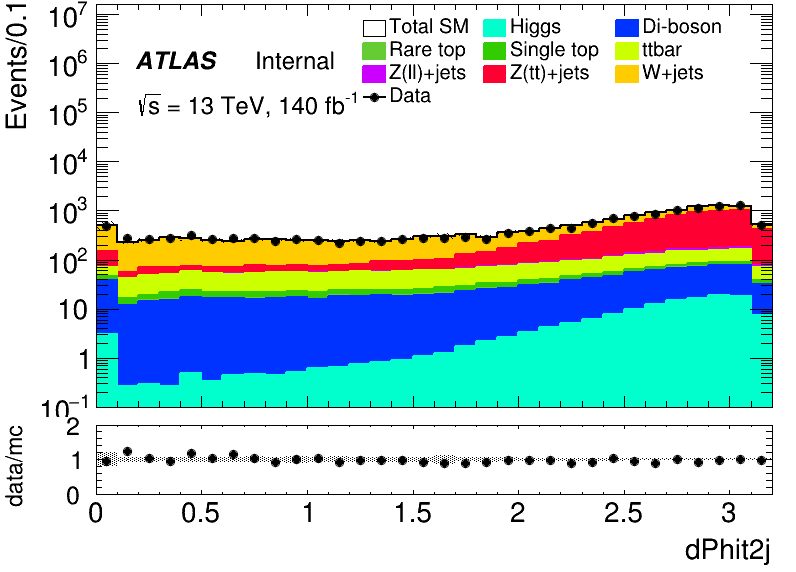
\includegraphics[width=\textwidth]{graphics/HH_met/HH_met_dPhit2j.png}
    \end{minipage}
    
    \vspace{0.5cm} % 图片之间的竖直间距

    % 第二行
    \begin{minipage}{0.32\textwidth}
        \centering
        \includegraphics[width=\textwidth]{graphics/HH_met/HH_met_dPhit2x.png}
    \end{minipage}
    \hfill
    \begin{minipage}{0.32\textwidth}
        \centering
        \includegraphics[width=\textwidth]{graphics/HH_met/HH_met_dPhixj.png}
    \end{minipage}
    \hfill
    \begin{minipage}{0.32\textwidth}
        \centering
        \includegraphics[width=\textwidth]{graphics/HH_met/HH_met_dPhitt.png}
    \end{minipage}
    notice: t1 is leading tau, t2 is next leading tau, j is leading jet, x is MET.
\end{frame}

\begin{frame}
\frametitle{C1N2ISR:MC modeling}
\framesubtitle{HH:\quad $\Delta R$}
% 第一行
    \begin{minipage}{0.32\textwidth}
        \centering
        \includegraphics[width=\textwidth]{graphics/HH_met/HH_met_dRt1j.png}
    \end{minipage}
    \hfill
    \begin{minipage}{0.32\textwidth}
        \centering
        \includegraphics[width=\textwidth]{graphics/HH_met/HH_met_dRt1x.png}
    \end{minipage}
    \hfill
    \begin{minipage}{0.32\textwidth}
        \centering
        \includegraphics[width=\textwidth]{graphics/HH_met/HH_met_dRt2j.png}
    \end{minipage}
    
    \vspace{0.5cm} % 图片之间的竖直间距

    % 第二行
    \begin{minipage}{0.32\textwidth}
        \centering
        \includegraphics[width=\textwidth]{graphics/HH_met/HH_met_dRt2x.png}
    \end{minipage}
    \hfill
    \begin{minipage}{0.32\textwidth}
        \centering
        \includegraphics[width=\textwidth]{graphics/HH_met/HH_met_dRxj.png}
    \end{minipage}
    \hfill
    \begin{minipage}{0.32\textwidth}
        \centering
        \includegraphics[width=\textwidth]{graphics/HH_met/HH_met_dRtt.png}
    \end{minipage}
    notice: t1 is leading tau, t2 is next leading tau, j is leading jet, x is MET.
\end{frame}

\begin{frame}
\frametitle{C1N2ISR:MC modeling}
\framesubtitle{HH:$\quad\eta$}
% 第一行
    \begin{minipage}{0.32\textwidth}
        \centering
        \includegraphics[width=\textwidth]{graphics/HH_met/HH_met_eta_jet.png}
    \end{minipage}
    \hfill
    \begin{minipage}{0.32\textwidth}
        \centering
        \includegraphics[width=\textwidth]{graphics/HH_met/HH_met_eta_lep.png}
    \end{minipage}
    \hfill
    \begin{minipage}{0.32\textwidth}
        \centering
        \includegraphics[width=\textwidth]{graphics/HH_met/HH_met_eta_tau.png}
    \end{minipage}
    notice: jet is leading jet, lep is next leading tau, tau is leading tau.
\end{frame}

\begin{frame}
\frametitle{C1N2ISR:MC modeling}
\framesubtitle{HH:\quad $p_t$}
% 第一行
    \begin{minipage}{0.32\textwidth}
        \centering
        \includegraphics[width=\textwidth]{graphics/HH_met/HH_met_pt_jet.png}
    \end{minipage}
    \hfill
    \begin{minipage}{0.32\textwidth}
        \centering
        \includegraphics[width=\textwidth]{graphics/HH_met/HH_met_pt_lep.png}
    \end{minipage}
    \hfill
    \begin{minipage}{0.32\textwidth}
        \centering
        \includegraphics[width=\textwidth]{graphics/HH_met/HH_met_pt_tau.png}
    \end{minipage}
    
    \vspace{0.5cm} % 图片之间的竖直间距
    notice: jet is leading jet, lep is next leading tau, tau is leading tau.
\end{frame}

\begin{frame}
\frametitle{C1N2ISR:MC modeling}
\framesubtitle{HH:\quad num}
% 第一行
    \begin{minipage}{0.32\textwidth}
        \centering
        \includegraphics[width=\textwidth]{graphics/HH_met/HH_met_nEles.png}
    \end{minipage}
    \hfill
    \begin{minipage}{0.32\textwidth}
        \centering
        \includegraphics[width=\textwidth]{graphics/HH_met/HH_met_nJets.png}
    \end{minipage}
    \hfill
    \begin{minipage}{0.32\textwidth}
        \centering
        \includegraphics[width=\textwidth]{graphics/HH_met/HH_met_nLeps.png}
    \end{minipage}
    
    \vspace{0.5cm} % 图片之间的竖直间距

    % 第二行
    \begin{minipage}{0.32\textwidth}
        \centering
        \includegraphics[width=\textwidth]{graphics/HH_met/HH_met_nMuons.png}
    \end{minipage}
    \hfill
    \begin{minipage}{0.32\textwidth}
        \centering
        \includegraphics[width=\textwidth]{graphics/HH_met/HH_met_nTaus.png}
    \end{minipage}
    \hfill
    \begin{minipage}{0.32\textwidth}
        \centering
        \includegraphics[width=\textwidth]{graphics/HH_met/HH_met_nTightTaus.png}
    \end{minipage}
\end{frame}

\begin{frame}
\frametitle{C1N2ISR:MC modeling}
\framesubtitle{HH:\quad transverse mass}
% 第一行
    \begin{minipage}{0.32\textwidth}
        \centering
        \includegraphics[width=\textwidth]{graphics/HH_met/HH_met_mt_jet.png}
    \end{minipage}
    \hfill
    \begin{minipage}{0.32\textwidth}
        \centering
        \includegraphics[width=\textwidth]{graphics/HH_met/HH_met_mt_lep.png}
    \end{minipage}
    \hfill
    \begin{minipage}{0.32\textwidth}
        \centering
        \includegraphics[width=\textwidth]{graphics/HH_met/HH_met_mt_tau.png}
    \end{minipage}
    
    \vspace{0.5cm} % 图片之间的竖直间距

    % 第二行
    \begin{minipage}{0.32\textwidth}
        \centering
        \includegraphics[width=\textwidth]{graphics/HH_met/HH_met_mtx_jet.png}
    \end{minipage}
        \hfill
    \begin{minipage}{0.32\textwidth}
        \centering
        \includegraphics[width=\textwidth]{graphics/HH_met/HH_met_mtx_lep.png}
    \end{minipage}
    \hfill
    \begin{minipage}{0.32\textwidth}
        \centering
        \includegraphics[width=\textwidth]{graphics/HH_met/HH_met_mtx_tau.png}
    \end{minipage}
    notice: mtx is the projection of MT in METvec.
\end{frame}
\begin{frame}
\frametitle{C1N2ISR:MC modeling}
\framesubtitle{HH:\quad stranverse mass, invariant mass, MET}
% 第一行
    \begin{minipage}{0.32\textwidth}
        \centering
        \includegraphics[width=\textwidth]{graphics/HH_met/HH_met_Mll.png}
    \end{minipage}
    \hfill
    \begin{minipage}{0.32\textwidth}
        \centering
        \includegraphics[width=\textwidth]{graphics/HH_met/HH_met_MT2.png}
    \end{minipage}
    \hfill
%    \begin{minipage}{0.32\textwidth}
%        \centering
%        \includegraphics[width=\textwidth]{graphics/H_met/H_met_dPhit2j.png}
%    \end{minipage}
    
    \vspace{0.5cm} % 图片之间的竖直间距

    % 第二行
    \begin{minipage}{0.32\textwidth}
        \centering
        \includegraphics[width=\textwidth]{graphics/HH_met/HH_met_MET.png}
    \end{minipage}
    \hfill
    \begin{minipage}{0.32\textwidth}
        \centering
        \includegraphics[width=\textwidth]{graphics/HH_met/HH_met_METsig.png}
    \end{minipage}
    \hfill
    
%    \begin{minipage}{0.32\textwidth}
%        \centering
%        \includegraphics[width=\textwidth]{graphics/H_met/H_met_dPhitt.png}
%    \end{minipage}

\end{frame}

\end{document}
